Zur Bestimmung der Übertragungskennlinien der Schaltkreisfamilien wurde das
Oszilloskop im XY-Modus konfiguriert, um Ein- und Ausgangsspannung direkt als
Kennlinie darstellen zu können. Zum Durchlauf der Eingangsspannungswerte wurde
eine Rampen-/Dreiecksfunktion an den jeweiligen Eingang gelegt (Abb. \ref{fig:triangle}) 

Es ergeben sich die Übertragungskennlinien aus
Abb. \ref{fig:first} und \ref{fig:last}

  \begin{figure}[H]
  \begin{center}
    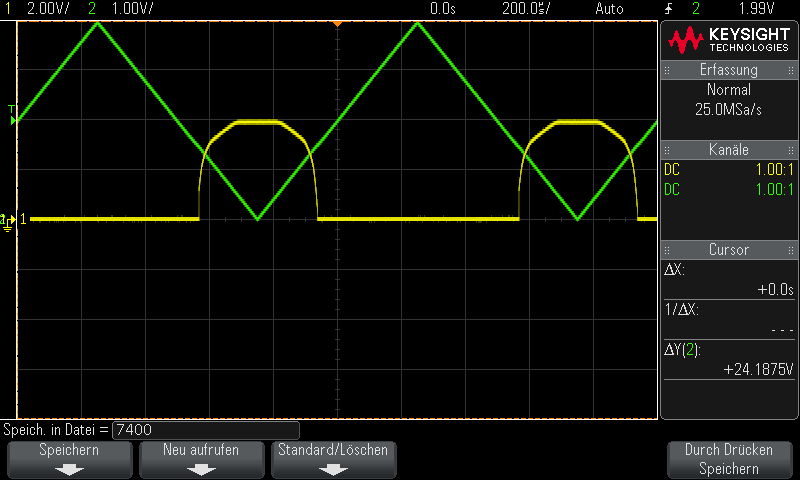
\includegraphics[width=\textwidth]{VERA/7400}
  \end{center}
  \caption{Ein-(Gelb) und Ausgangsspannung (Grün, 7400) in der normalen Zeitdarstellung}
  \label{fig:triangle2}
\end{figure}

  \begin{figure}[H]
  \begin{center}
    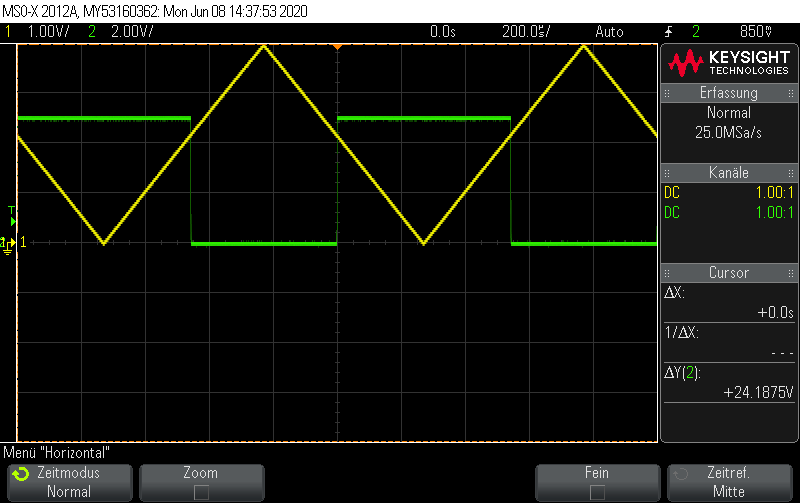
\includegraphics[width=\textwidth]{VERA/74111}
  \end{center}
  \caption{Ein-(Gelb) und Ausgangsspannung (Grün, 4011) in der normalen Zeitdarstellung}
  \label{fig:triangle}
\end{figure}

  \begin{figure}[H]
  \begin{center}
    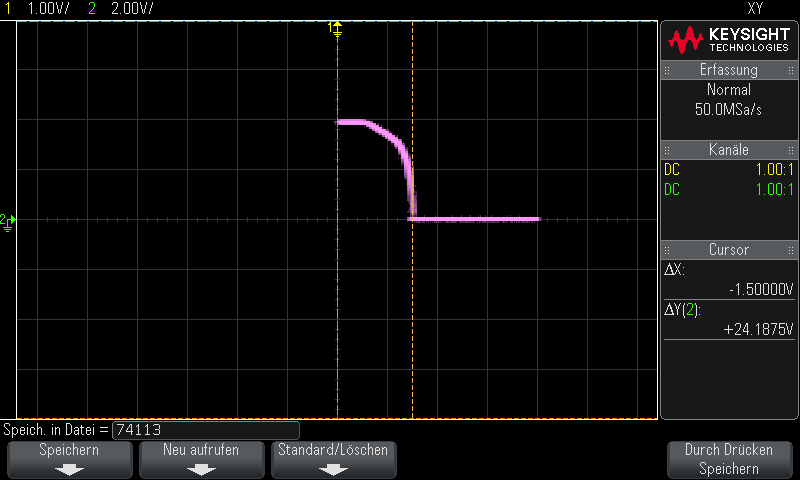
\includegraphics[width=\textwidth]{VERA/74113}
  \end{center}
  \caption{Übertragungskennlinie des 7400 TTL-Gatters}
  \label{fig:first}
\end{figure}

  \begin{figure}[H]
  \begin{center}
    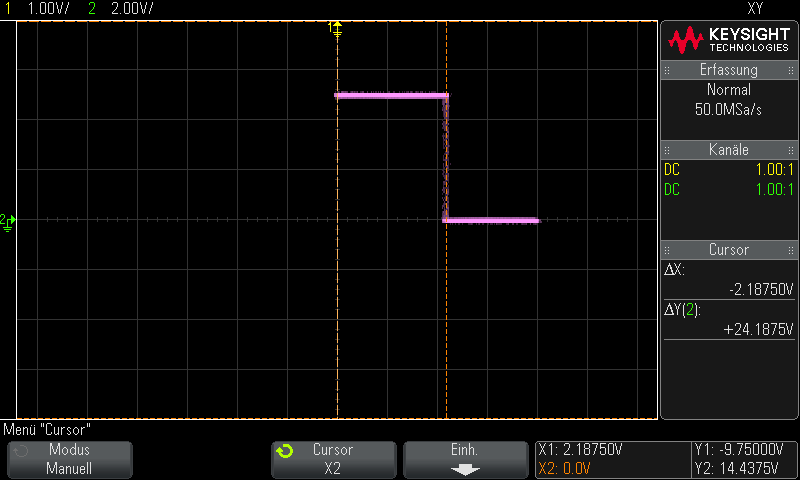
\includegraphics[width=\textwidth]{VERA/74112}
  \end{center}
  \caption{Übertragungskennlinie des 4011 CMOS-Gatters}
  \label{fig:last}
\end{figure}

Man erkennt die gewöhnliche \glqq Stufung\grqq in der Übertragungskennlinie des
7400 TTL-Gatters. Die Kennlinie des CMOS-Gatters enthält, wie erwartet, einen
steileren Übergang und somit eine diskretere Unterscheidung zwischen HIGH-und
LOW (Cursor zeigen die Schaltschwellen).

